%-----------------------------------------------------------------------------
%	PACKAGES AND DOCUMENT CONFIGURATIONS
%-----------------------------------------------------------------------------

\documentclass{article}

\usepackage{graphicx} % Required for the inclusion of images
\usepackage{natbib} % Required to change bibliography style to APA
\usepackage{amsmath} % Required for some math elements
\usepackage{amssymb}
\usepackage{grffile}
\usepackage[export]{adjustbox}
\usepackage{subcaption}
\usepackage{float}
\usepackage{listings}
\usepackage[margin=1.0in]{geometry}
\usepackage{tikz}
\usepackage{enumitem}
\usepackage{scrextend}
\usepackage{siunitx}
\usepackage{minted}

\usetikzlibrary{shapes.geometric, arrows}
\tikzstyle{startstop} = [rectangle, rounded corners, minimum width=1cm, minimum height=1cm,text centered, draw=black, fill=white!30]
\tikzstyle{process} = [rectangle, minimum width=1cm, minimum height=1cm, text centered, draw=black, fill=white!30]
\tikzstyle{arrow} = [thick,->,>=stealth]

\setlength\parindent{0pt} % Removes all indentation from paragraphs

%-----------------------------------------------------------------------------
%	DOCUMENT INFORMATION
%-----------------------------------------------------------------------------

\title{ECE 547 Fall 2016 Homework 3} % Title

\author{Yang \textsc{Wang}}  % Author name

\date{\today} % Date for the report

\renewcommand{\theenumi}{\alph{enumi}} % use letters for list items

\begin{document}

\maketitle % Insert the title, author and date

%-----------------------------------------------------------------------------
%	Problem 1
%-----------------------------------------------------------------------------

\section*{Analytical Questions}
	\subsection*{Problem 1}

		Propagation Delay: the amount of time needed for traveling to McDonald's and
		back to the office. \\
		Transmission Delay: the amount of time needed for consuming the food. \\
		Processing Delay: the amount of time needed for choosing the meal. \\
		Queueing Delay: the amount of time needed for waiting up in line to order.

	\subsection*{Problem 2}
		\subsubsection*{Deriving I from II}
			From Definition I, we have $P(\left\{ N(t) = 1 \right\}) = \lambda t + o(t)$.
			And from Definition II, we have,
			\begin{align*}
				P(\left\{ N(t) = 1 \right\}) &= e^{-\lambda t} \frac{(\lambda t)^1}{1!} \\
				&= \lambda t (1 - \lambda t + \frac{(\lambda t)^2}{2!} + \ldots ) \\
				&= \lambda t + o(t)
			\end{align*}
			In addition, from Definition I, we have $P(\left\{ N(t) \geqslant 2 \right\}) = o(h)$.
			Using Defintion II, we have,
			\begin{align*}
				P(\left\{ N(t) \geqslant 2 \right\}) &= \sum_{n=2}^{\infty} e^{-\lambda t} \frac{(\lambda t)^n}{n!} \\
				&= e^{\lambda t} (\frac{(\lambda t)^2}{2!} + \frac{(\lambda t)^3}{3!} + \ldots) \\
				&= o(t)
			\end{align*}
			Hence, Definition I  and II are equivalent.
		\subsubsection*{Deriving II from I}
			Using the hint provided, we have,
			\begin{gather*}
				\frac{P_{0}(t+h) - P_{0}(t)}{h} = -\lambda P_{0}(t) + \frac{o(h)}{h}
			\end{gather*}
			As h goes to 0, we can have,
			\begin{align*}
				\frac{dP_{0}(t)}{dt} &= -\lambda P_{0}(t) \\
				\implies P_{0}(t) &= e^{-\lambda t}
			\end{align*}
			Now we need to solve the case when $n \geqslant 1$.
			\begin{align*}
				P_{n}(t+h) &= P(\left\{ N(t) = n, N(t+h) - N(t) = 0 \right\}) \\
				&+ P(\left\{ N(t) = n - 1, N(t+h) - N(t) = 1 \right\}) \\
				&+ P(\left\{ N(t) = n, N(t+h) - N(t) \geqslant 2 \right\}) \\
				&= P_{n}(t)P_{0}(h) + P_{n-1}(t)P_{1}(h) + o(h) \\
				&= (1 - \lambda h)P_{0}(t) + \lambda h P_{n-1}(t) + o(h) \\
				\implies \frac{P_{n}(t+h) - P_{n}(t)}{h} &= -\lambda P_{n}(t) + \lambda P_{n-1}(t) + \frac{o(h)}{h}
			\end{align*}
			As h goes to 0, we have this differential equation,
			\begin{align*}
				\frac{dP_{n}(t)}{dt} &= -\lambda P_{n}(t) + \lambda P_{n-1}(t)
			\end{align*}
			By solving this equation, we got,
			\begin{align*}
				P_{n}(t) = e^{-\lambda t} \frac{(\lambda t)^n}{n!}
			\end{align*}
			Hence, Definition I and II are equivalent.

	\subsection*{Problem 3}

		Let $A = \left\{ \text{one packet arrive at the node successfully} \mid \text{packet has length } n \right\}$,
		\begin{gather*}
			\implies P(A) = (1-p)^{n}
		\end{gather*}

		Let $B = \left\{ \text{packets arrive at the node successfully} \right\}$
		and $C = \left\{ \text{packet has length } n \right\} $,
		\begin{align*}
			\implies P(B) &= \sum_{n = 0}^{\infty} P(A) \cdot P(C) \\
			&= \sum_{n = 0}^{\infty} (1-p)^{n} \frac{\mu^{n}e^{-\mu}}{n!} \\
			&= e^{-\mu} \sum_{n = 0}^{\infty} (1-p)^{n} \frac{\mu^{n}}{n!} \\
			&= e^{-\mu p} \sum_{n = 0}^{\infty} e^{-\mu (1-p)} \frac{((1-p)\mu)^{n}}{n!} \\
			&= e^{-\mu p} \cdot 1 \\
			&= e^{-\mu p}
		\end{align*}

		Therefore, the rate at which succcessful packets arrive the network node is:
		\begin{align*}
			\text{rate} = e^{-\mu p} \cdot \lambda
		\end{align*}

	\subsection*{Problem 4}

		We are given that $\tau_{1}$ and $\tau_{2}$ are independent, exponential
		distribution with mean $\frac{1}{\lambda_{1}}$ and $\frac{1}{\lambda_{2}}$.
		Therefore, we can write,
		\begin{align*}
			P(\left\{ \tau_{1}  \geqslant t \right\}) &= e^{-\lambda_{1} t} \\
			P(\left\{ \tau_{2}  \geqslant t \right\}) &= e^{-\lambda_{2} t}
		\end{align*}
		We can also write,
		\begin{align*}
			P(\left\{ \text{min}(\tau_{1}, \tau_{2}) \right\}) &= P(\left\{ \tau_{1} \geqslant t, \tau_{2} \geqslant t  \right\}) \\
			&= P(\left\{ \tau_{1} \geqslant t \right\}) \cdot P(\left\{ \tau_{2} \geqslant t \right\}) \\
			&= e^{-(\lambda_{1} + \lambda_{2})t}
		\end{align*}
		Hence, we can say that r.v. min$(\tau_{1}, \tau_{2})$ is exponentially
		distributed with mean $\frac{1}{\lambda_{1} + \lambda_{2}}$.

		For showing $P(\left\{ \lambda_{1} < \lambda_{2} \right\}) = \frac{\lambda_{1}}{\lambda_{1} + \lambda_{2}}$,
		we first know the event $\left\{ \lambda_{1} < \lambda_{2} \right\}$ is
		equivalent as $\left\{ \lambda_{1} < t \mid t = \lambda_{2} \right\}$. Hence,
		we can write,
		\begin{align*}
			P(\left\{ \lambda_{1} < \lambda_{2} \right\}) &= P(\left\{ \lambda_{1} < t \mid t = \lambda_{2} \right\}) \\
			&= \int_{0}^{\infty} P(\left\{ \lambda_{1} < t \right\}) f_{\tau_{2}}(t)dt \\
			&= \int_{0}^{\infty} (1 - e^{-\lambda_{1}t}) \lambda_{2}e^{-\lambda_{2}t}dt \\
			&= \lambda_{2} \int_{0}^{\infty} (1 - e^{-\lambda_{1}t}) e^{-\lambda_{2}t}dt \\
			&= \lambda_{2} \int_{0}^{\infty} (e^{-\lambda_{2}t} - e^{-(\lambda_{1} + \lambda_{2})})dt \\
			&= \lambda_{2} (\frac{e^{-\lambda_{2}t}}{\lambda_{2}} - \frac{e^{-(\lambda_{1} + \lambda_{2})}}{-(\lambda_{1} + \lambda_{2})}) \bigg|_{0}^{\infty} \\
			&= 1 - \frac{\lambda_{2}}{\lambda_{1} + \lambda_{2}} \\
			&= \frac{\lambda_{1}}{\lambda_{1} + \lambda_{2}}
		\end{align*} 
	\subsection*{Problem 5}
		\subsubsection*{Schwartz 2-6}
			\begin{enumerate}
				\item We need to obatin $(\lambda + \mu) p_{n} = \lambda p_{n-1} + \mu p_{n+1}$
					for $n \geqslant 1$. From Schwartz 2-12, we already have,
					\begin{gather*}
						p_{n}(t + \Delta t) = p_{n}(t) [ (1 - \lambda \Delta t)(1 - \mu \Delta t) + \mu \Delta t \cdot \lambda \Delta t + o(\Delta t) ] \\
						+ p_{n-1}(t) [ \lambda \Delta t (1 - \mu \Delta t) + o(\Delta t) ] \\
						+ p_{n+1}(t) [ \mu \Delta t (1 - \lambda \Delta t) + o(\Delta t) ]
					\end{gather*}
					We can factor the $(\Delta t)^{2}$ terms into $o(\Delta t)$ since they
					are usually very small,
					\begin{gather*}
						\implies p_{n}(t + \Delta t) = p_{n}(t) [1 - (\lambda + \mu) \Delta t] + p_{n-1}(t) (\lambda \Delta t) + p_{n+1}(t) (\mu \Delta t)
					\end{gather*}
					From Taylor Series,
					\begin{align*}
						p_{n}(t + \Delta t) &= p_{n}(t) + \frac{dp_{n}(t)}{dt} \Delta t \\
						\implies \frac{dp_{n}(t)}{dt} &= (-\lambda + \mu) p_{n}(t) + \lambda p_{n-1}(t) + \mu p_{n+1}(t)
					\end{align*}
					We want to find the steady state value of $p_{n}$, hence by setting $\frac{dp_{n}(t)}{dt} = 0$,
					\begin{align*}
						(\lambda + \mu) p_{n} = \lambda p_{n-1} + \mu p_{n+1}, n \geqslant 1
					\end{align*}
				\item From Fig. 2-11 in Schwartz textbook, we can use the Conservation
					of Rates (i.e., the rate going \textbf{in} a node equals to the rate
					going \textbf{out} of a node) to set up our equation which is just,
					\begin{align*}
						p_{n-1}\lambda + p_{n+1}\mu = p_{n}(\lambda + \mu)
					\end{align*}
			\end{enumerate}
		\subsubsection*{Schwartz 2-8}
			For the M/M/1 queue analysis, we have the stationary state probability $p_{n} = \rho^{n} p_{0}$,
			where $\rho = \frac{\lambda}{\mu}$.
			\begin{enumerate}
				\item Show that the stationary state probability satisfies Eq. 2-15.
					We can plug in the stationary state probability $p_{n} = \rho^{n} p_{0}$
					into Eq. 2-15 to verify the equation holds:
					\begin{align*}
						(\lambda + \mu) p_{n} &= \mu \rho^{n+1} p_{0} + \lambda \rho^{n-1} p_{0} \\
						&= \mu p_{n+1} + \lambda p_{n-1}
					\end{align*}
					Hence, $p_{n}$ satisfies Eq. 2-15.
				\item For showing $\lambda p_{n} = \mu p_{n+1}$ satifies Eq. 2-15, we
					can first start by examining Eq. 2-15,
					\begin{align*}
						(\lambda + \mu) p_{n} &= \lambda p_{n-1} + \mu p_{n+1} \\
						\implies \lambda p_{n} - \mu p_{n+1} &= \lambda p_{n-1} - \mu p_{n}
					\end{align*}
					As proved in class, $\lambda p_{n-1} - \mu p_{n} = 0$, hence,
					\begin{gather*}
						\lambda p_{n} - \mu p_{n+1} = 0 \\
						\implies \lambda p_{n} = \mu p_{n+1} 
					\end{gather*}
					As a result, the stationary state probability satisfies Eq. 2-15.
				\item We need to calculate $p_{0}$ for the M/M/1/N queu and show that $p_{n}$
					is given by Eq. 2-20 in Schwartz.
					From the class notes, we already showed that the stationary state
					probability for M/M/1/N queue is $p_{n} = (\frac{\lambda}{\mu})^n p_{0}$,
					therefore, by normalizing $p_{n}$, we get,
					\begin{align*}
						\sum_{n=0}^{N} p_{n} &= \sum_{n=0}^{N} (\frac{\lambda}{\mu})^n p_{0} \\
						&= p_{0} \sum_{n=0}^{N} \rho^{n} \\
						&= p_{0} \frac{1 - \rho^{N+1}}{1 - \rho} \\
						&= 1
					\end{align*}
					Hence,
					\begin{gather*}
						p_{0} = (\frac{1 - \rho^{N+1}}{1 - \rho})^{-1}
					\end{gather*}
					We can then substitute $p_{0}$ into the stationary state probability
					to obatin Eq. 2-20.
			\end{enumerate}

\section*{Simulation-Based Experiments}
	\subsection*{Problem 1}
		\begin{figure}[!hbt]
			\centering
			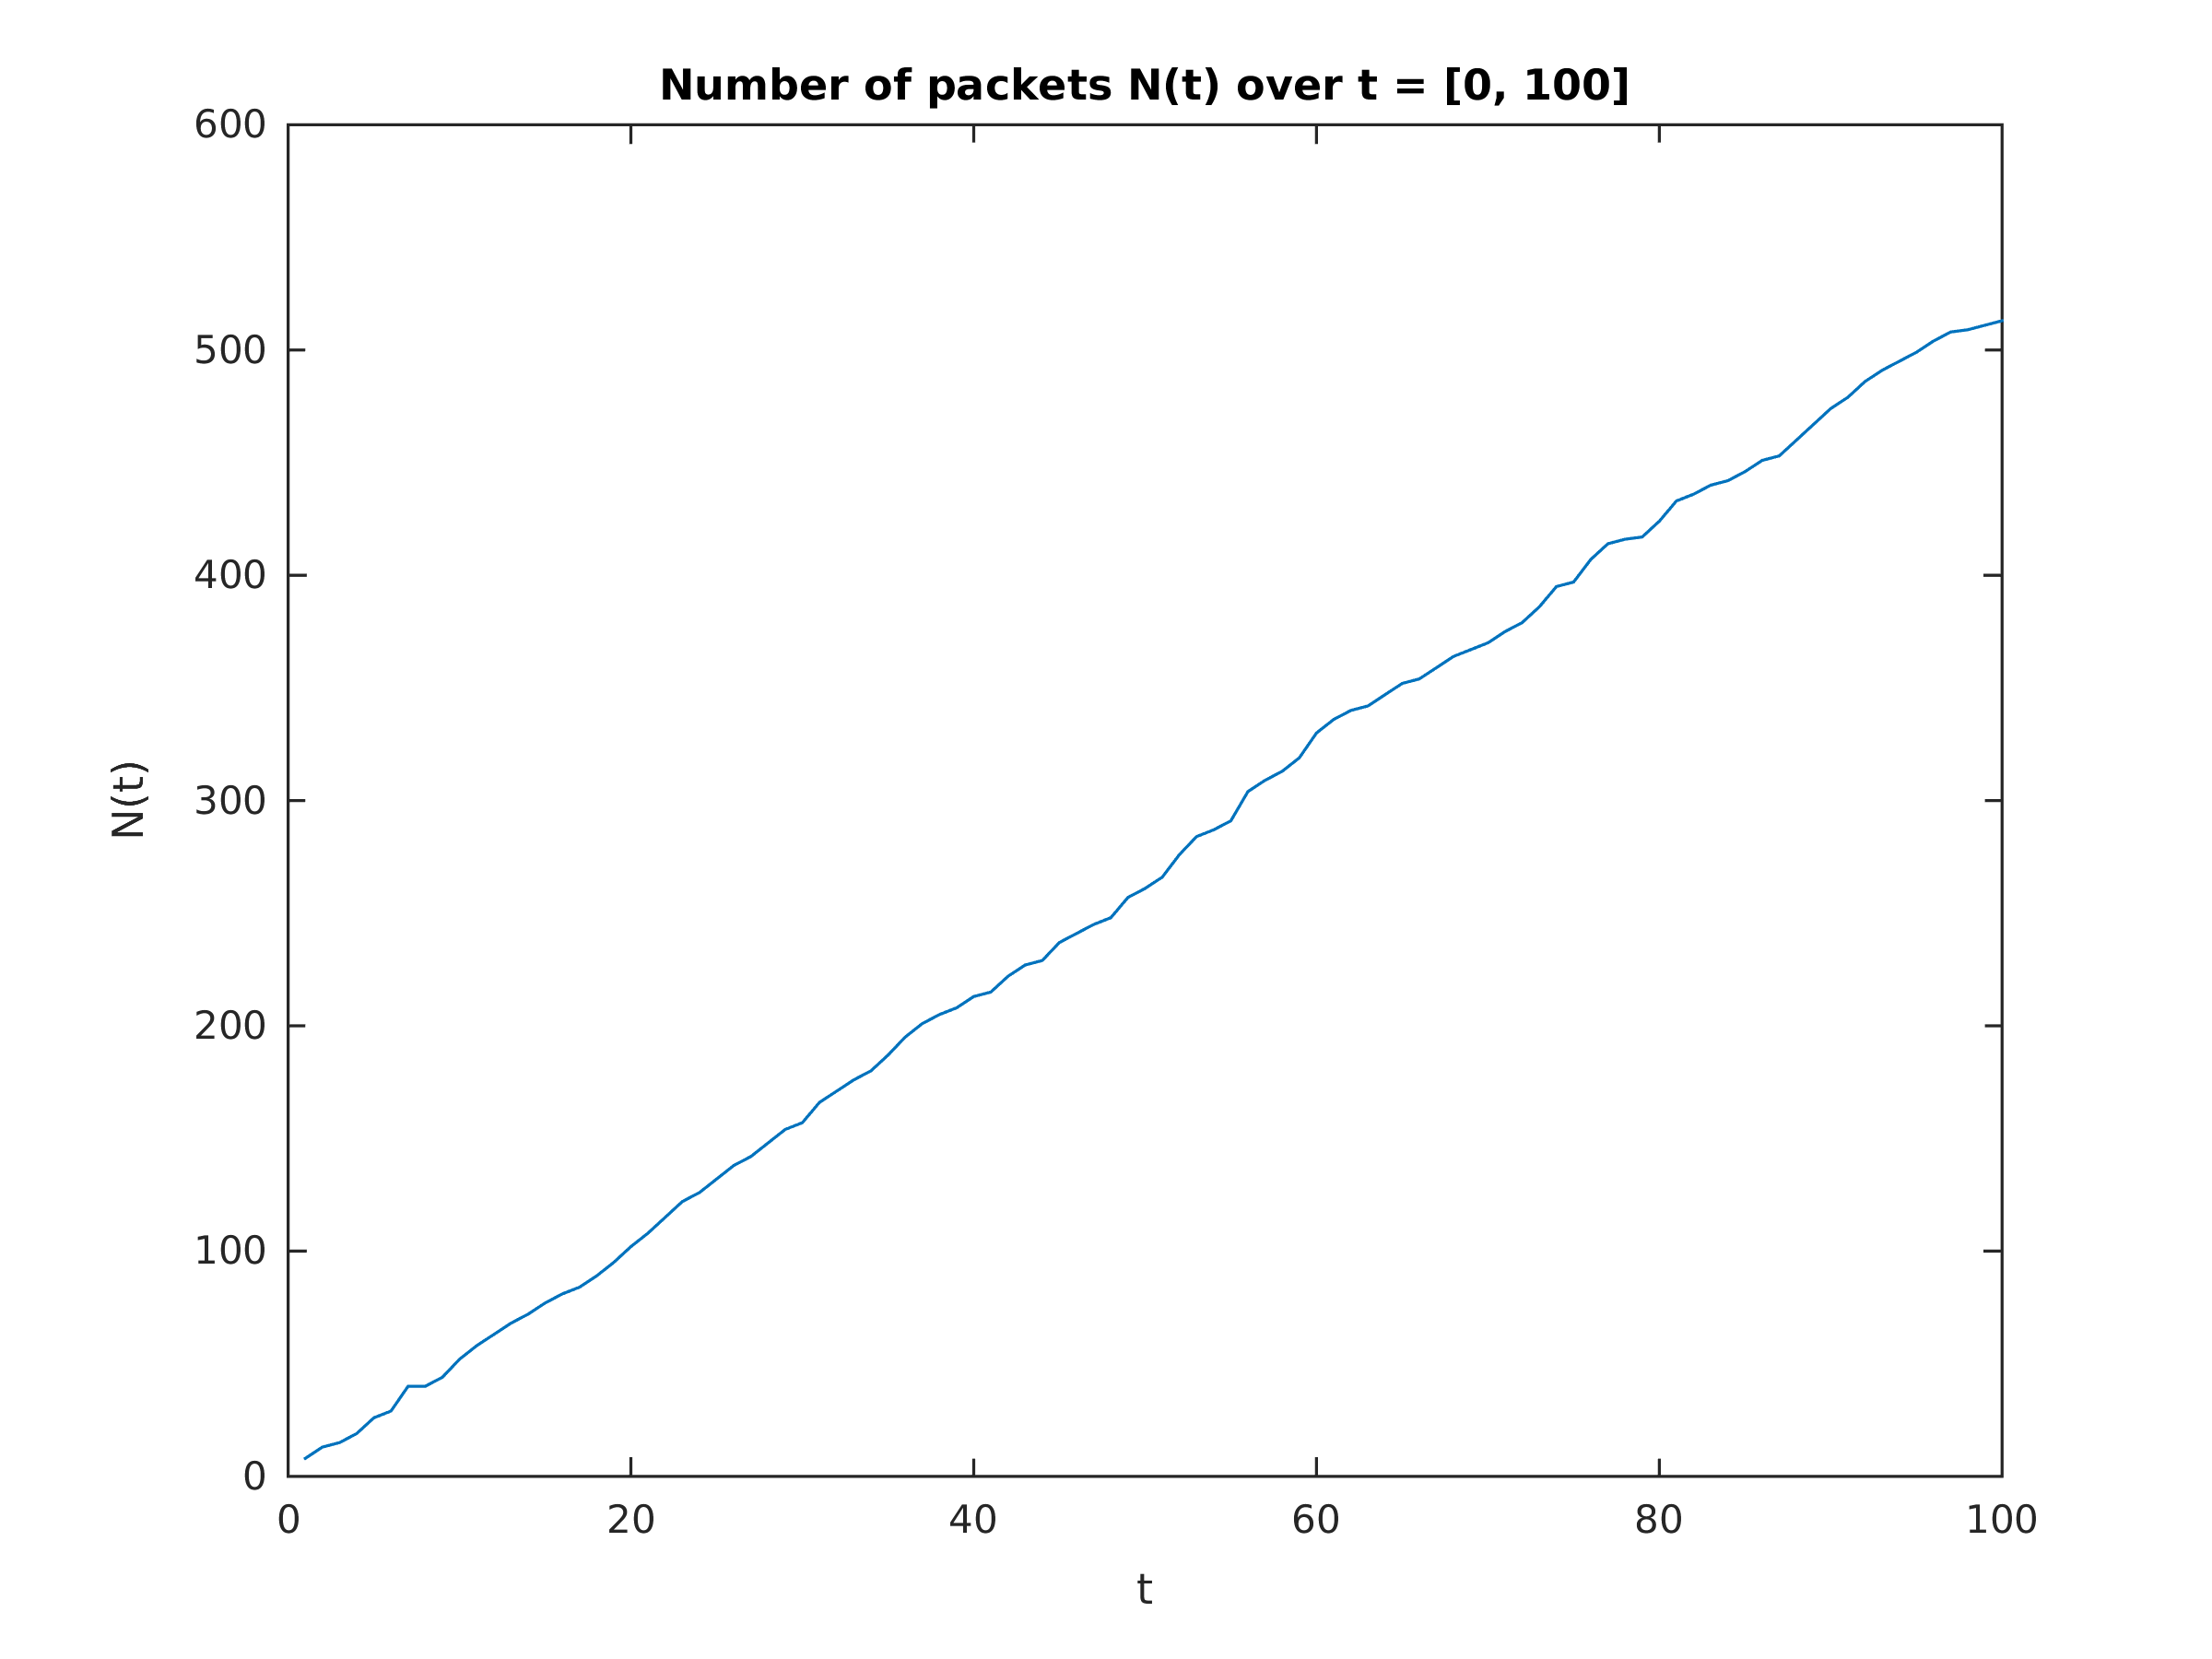
\includegraphics[width=0.5\linewidth]{hw3_1_nt.png}
			\caption{Poisson process $N(t)$ over t = [0, 100] when $\lambda=5$}
		\end{figure}

		We already know that the inter-arrival time is exponentially distributed.
		Hence, for generating a Poisson process, one way is to generate the arrival
		times when arrival occurs. When we obtain the event times, we can find the
		corresponding number of arrivals given a time $t$. A couple of values of $t$
		are used to simulate the Poisson process but only when $t=100$ is given in
		Figure 1. The pattern is rather clear: N(t) converges to a large number as t
		goes to infinity.

	\subsection*{Problem 2}
		\begin{figure}[!hbt]
			\centering
			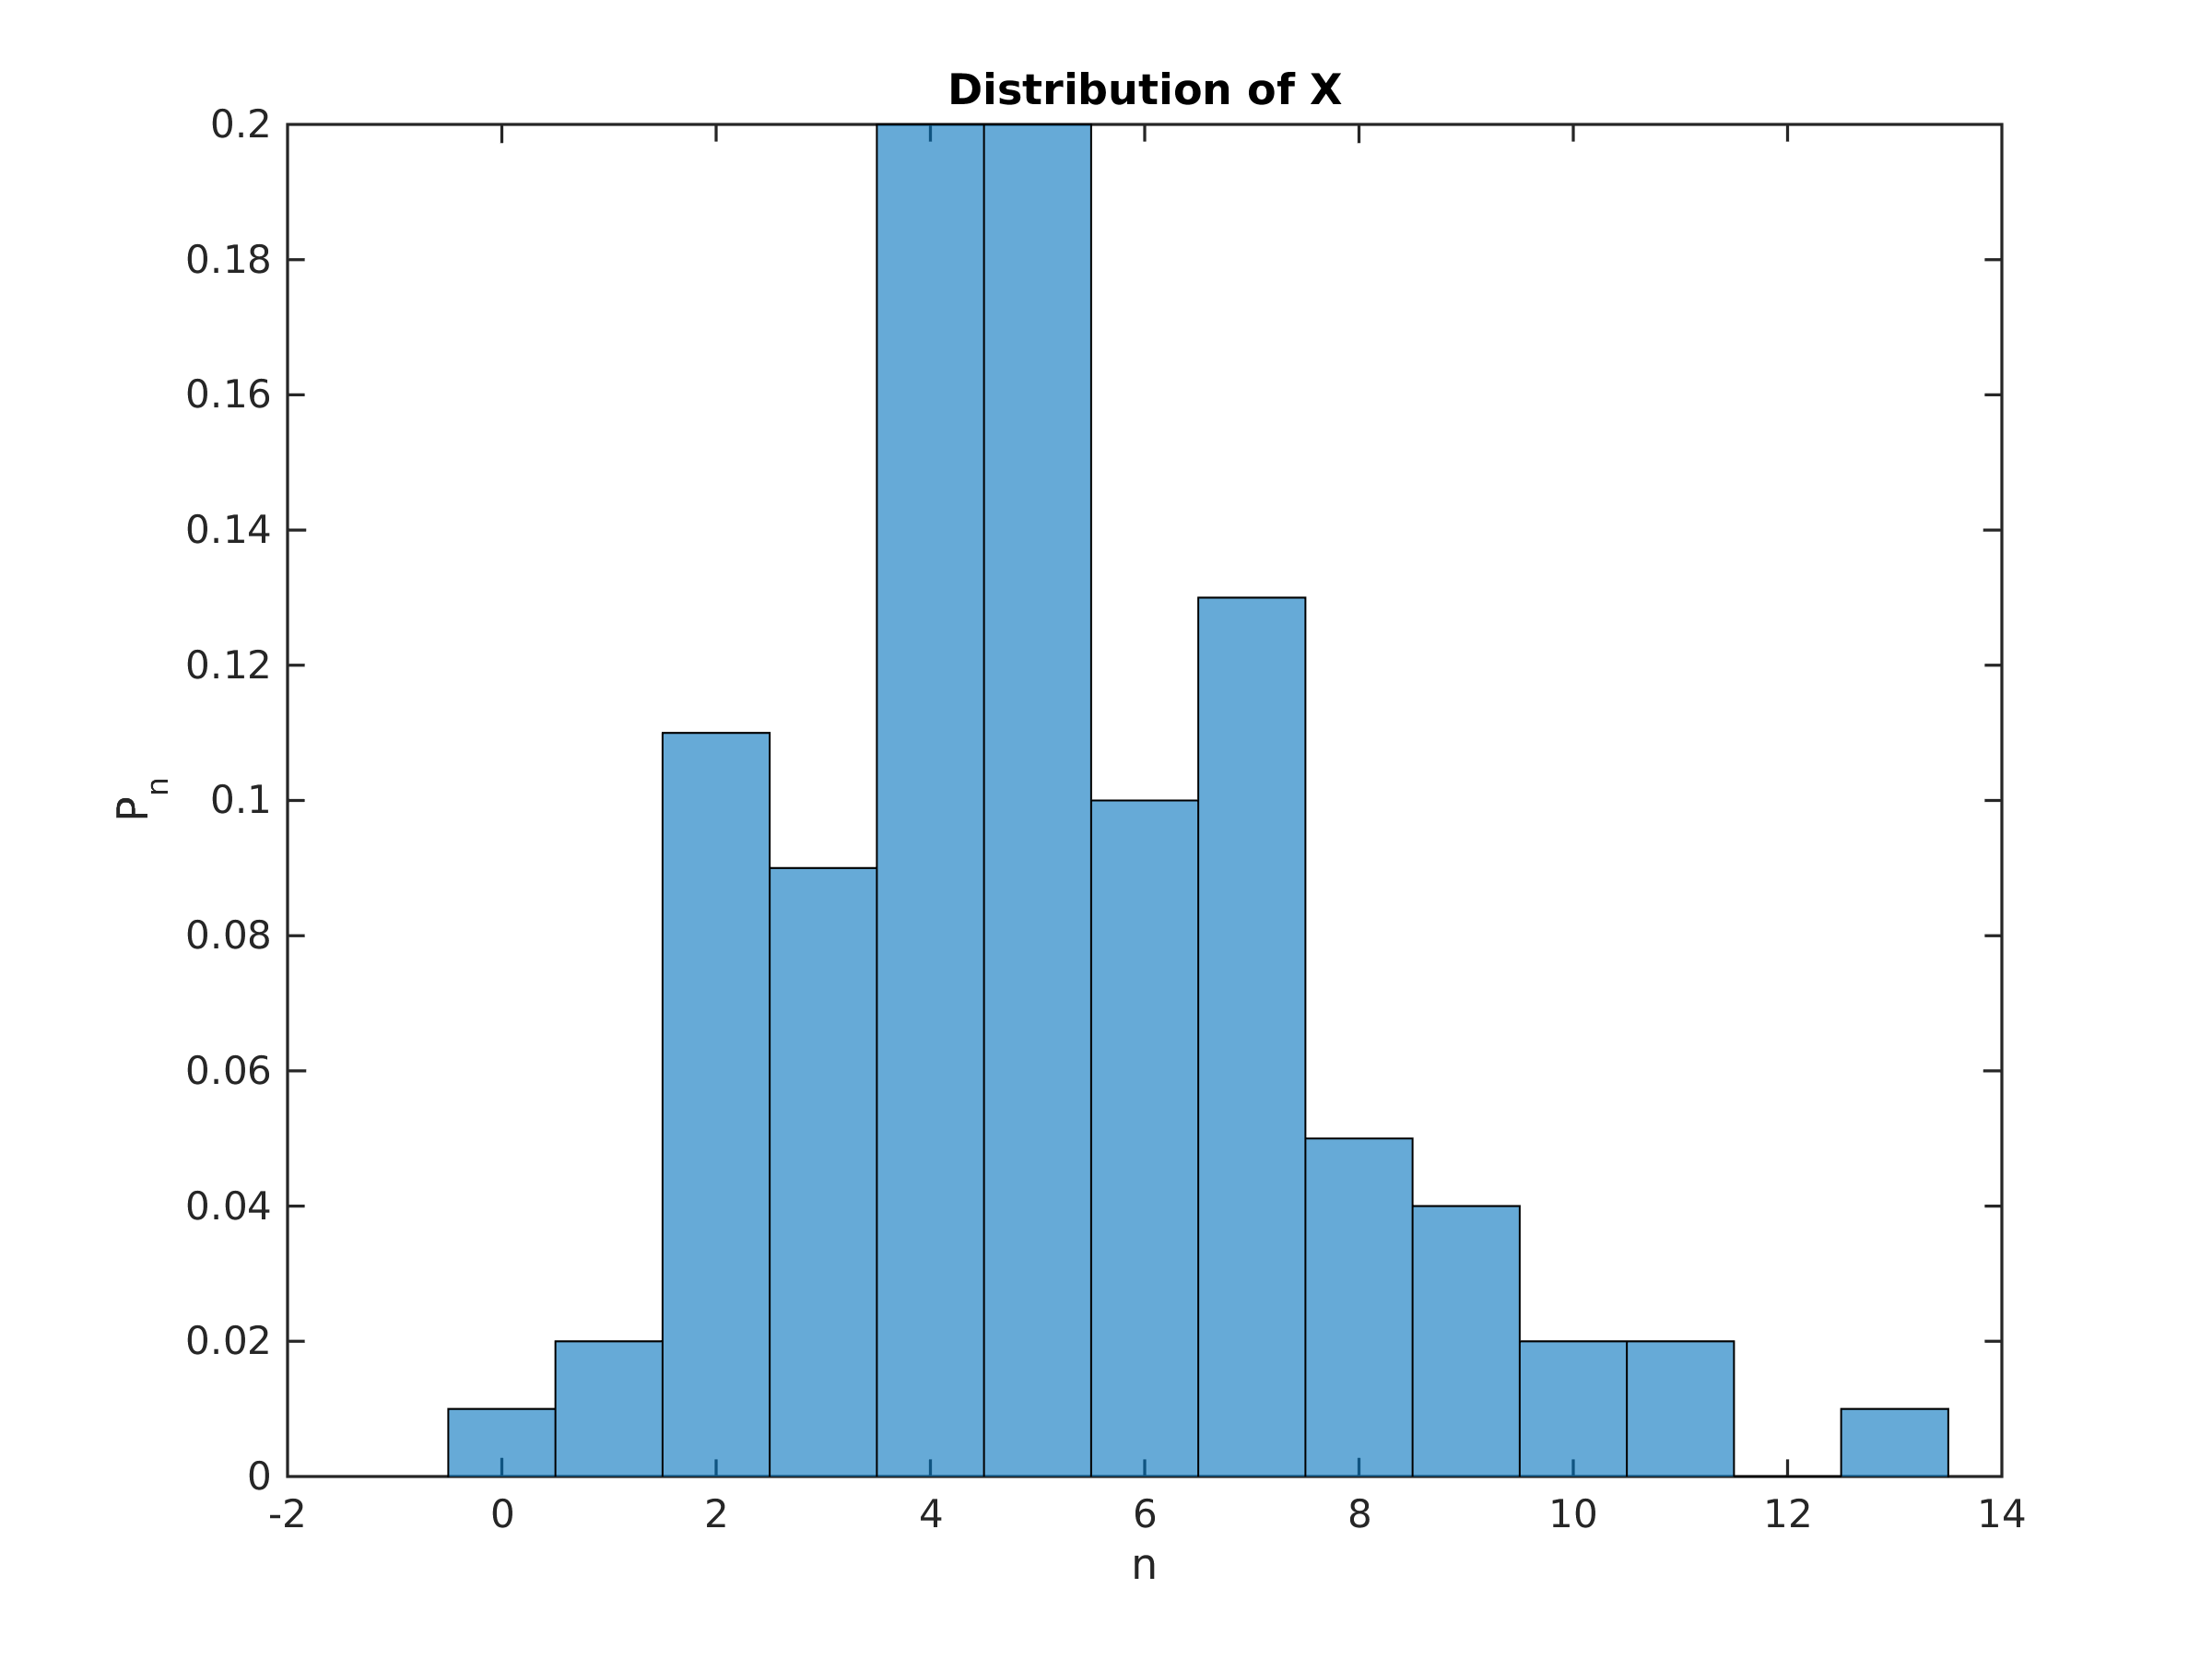
\includegraphics[width=0.5\linewidth]{hw3_2_pn.png}
			\caption{Verification of r.v. $X$ is Poisson distributed.}
		\end{figure}

		From the MATLAB simulations, we get $E[X]=5.1300$. We can further verify
		that $X$ is a Poisson distribution by plotting its distribution as in
		Figure 2.

	\subsection*{Problem 3}
		The problem essentially requires us to simulate the M/M/1 queueing system.
		At first glance, we have a fixed arrival rate of $\lambda=5$ and three
		different service rate $\mu$ values which are 4, 6, and 10. Intuitively,
		since the system has 1 server and an infinite buffer. When $\mu = 4$, that
		means the service rate cannot keep up with the arrival rate, hence, the
		packets in the infinite buffer will build up to a very large number. On the
		other hand, for $\mu = 10$, the service rate is twice as big as the arrival
		rate, hence, for every packet that arrives into the system, the packet is
		served immediately and hence, no buffer space is filled which infers that
		the average number of packets will be very low (approximately 0). When $\mu = 6$,
		the system will follow very closely to a Poisson process and the average
		number of packets should be bigger than 0 but much less than when $\mu = 4$.
		We can verify our intuitions by simulating the M/M/1 queue using different
		values of $\mu$. Please see the figures on the next page. Also from MATLAB
		simulation results,
		\begin{gather*}
			E[n]_{\mu = 6} = 2.0918 \\ 
			E[n]_{\mu = 4} = 1884.9 \\ 
			E[n]_{\mu = 10} = 0 
		\end{gather*}

		\begin{figure}[!hbt]
			\centering
			\begin{subfigure}[!hbt]{0.45\linewidth}
				\centering
				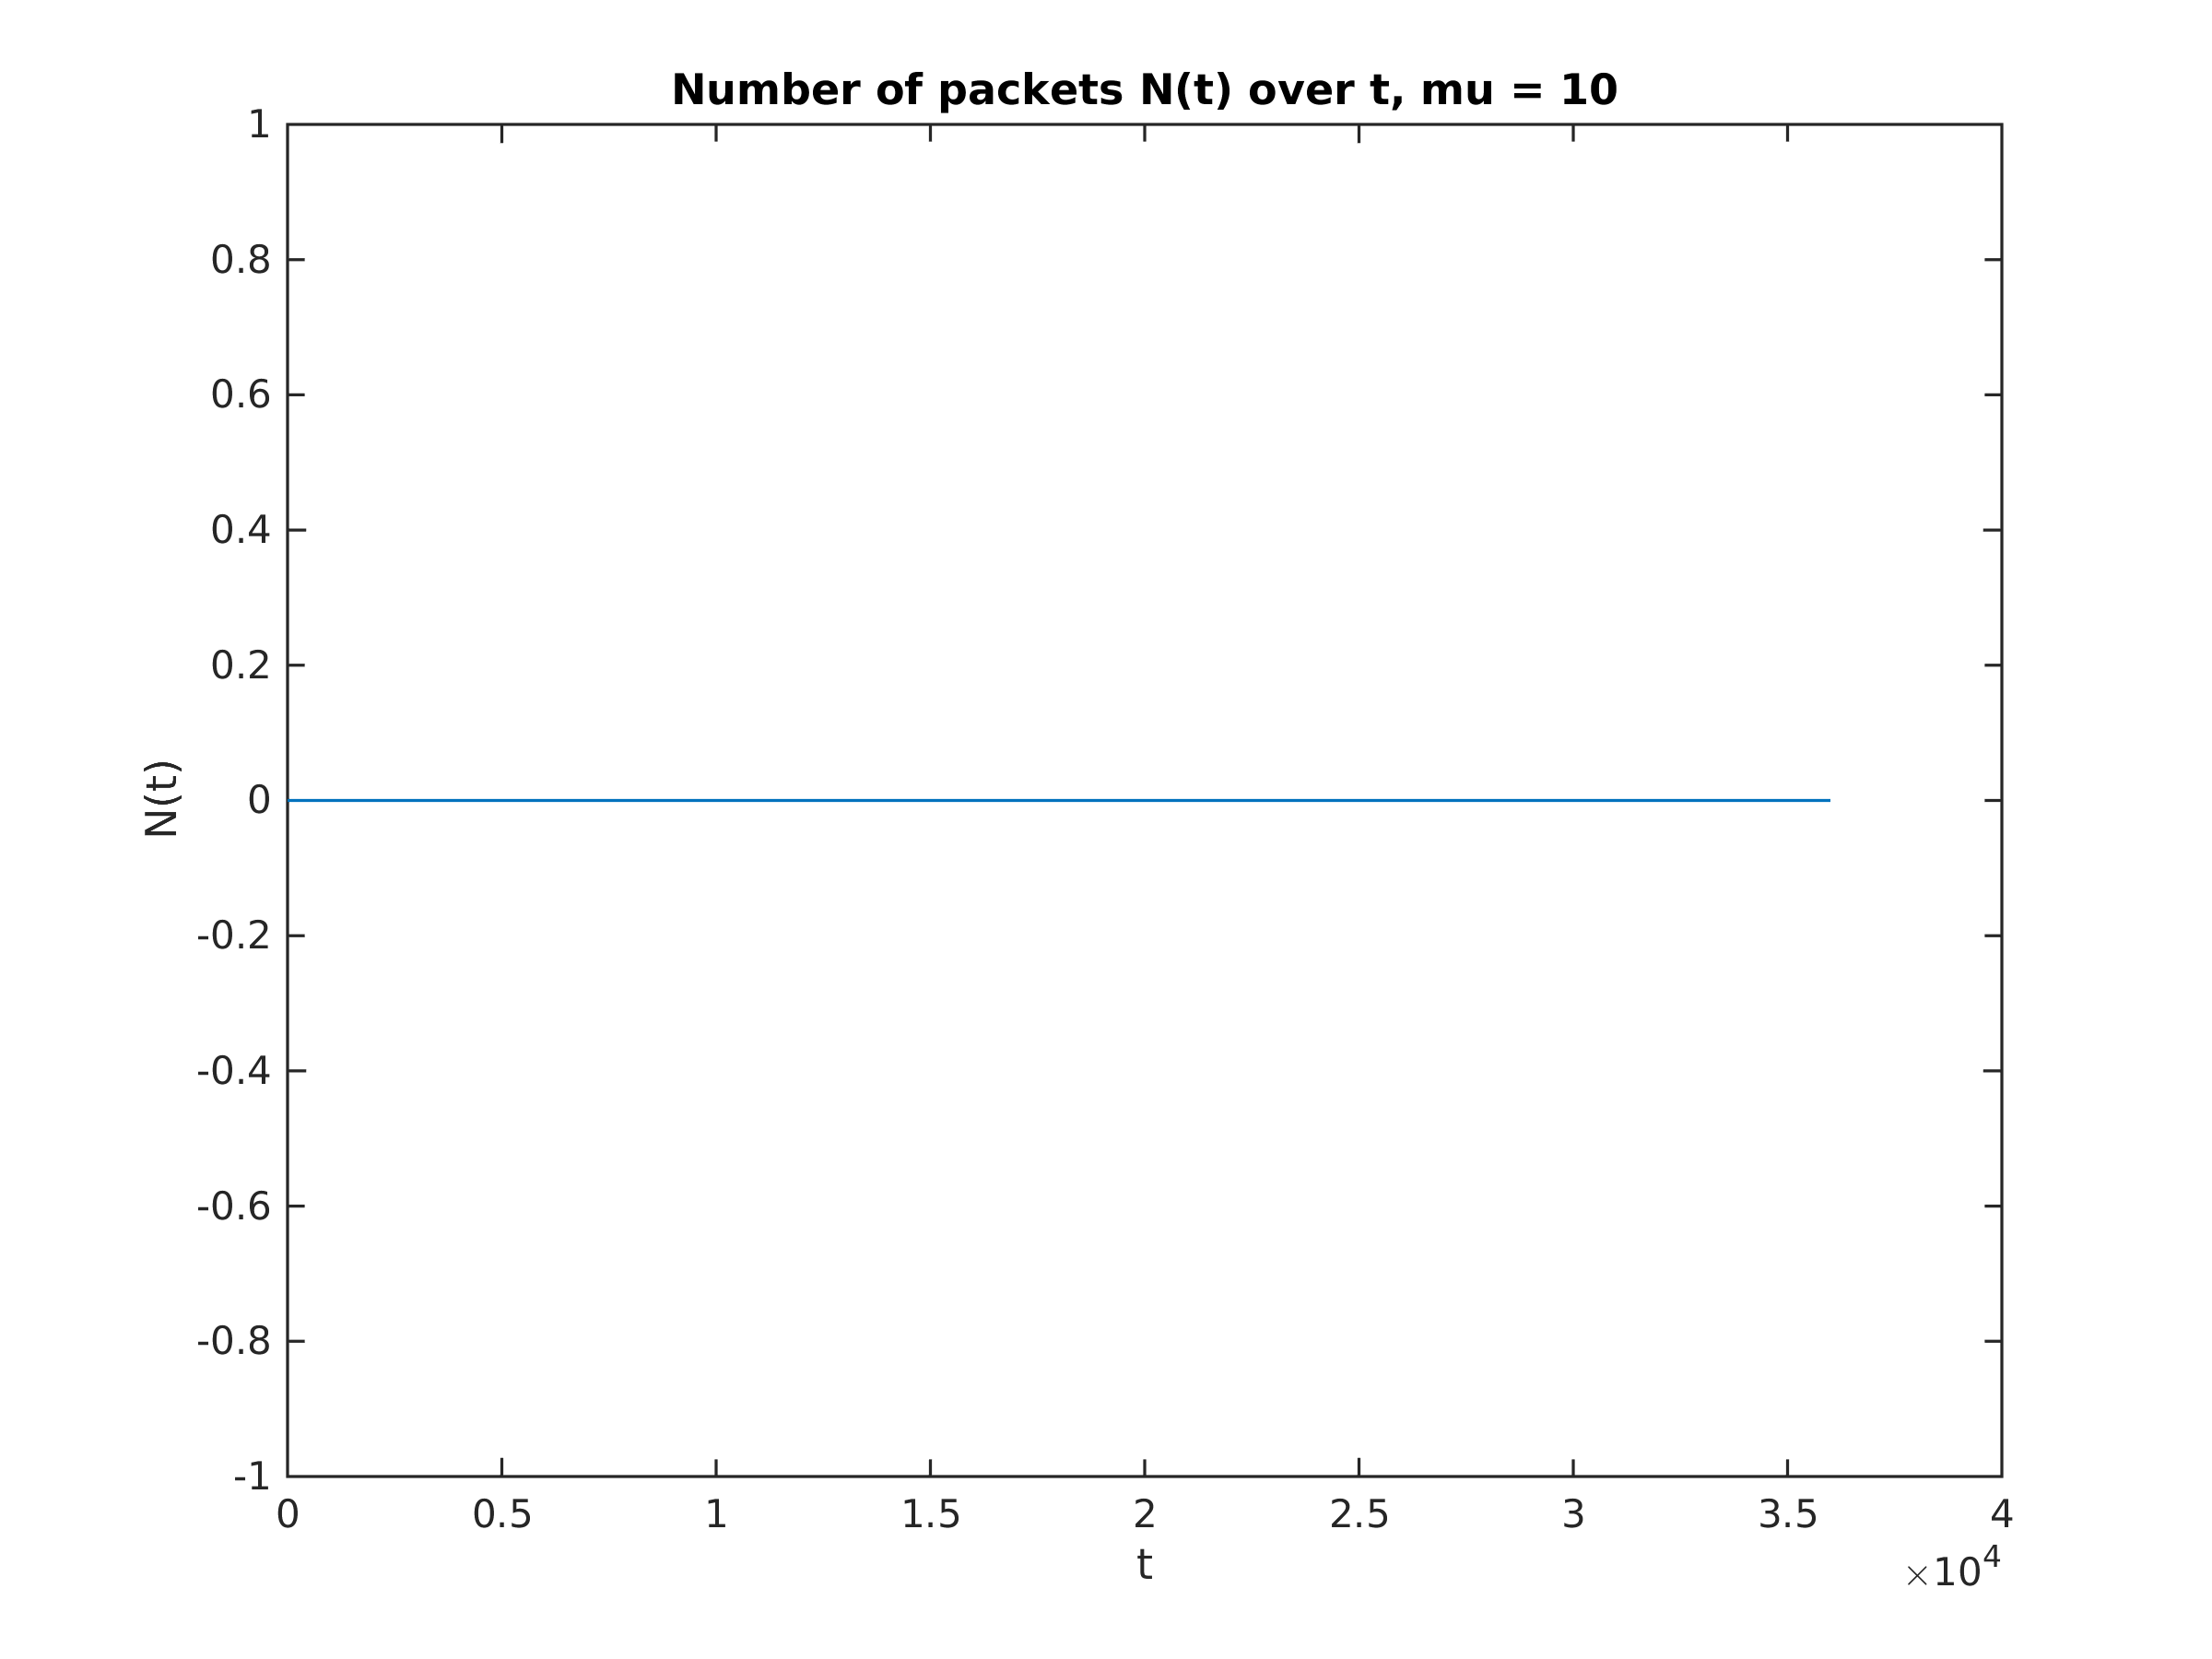
\includegraphics[width=1\linewidth]{hw3_3_nt_m10.png}
				\caption{$n(t)$ when $\mu = 10$.}
			\end{subfigure}
			\begin{subfigure}[!hbt]{0.45\linewidth}
				\centering
				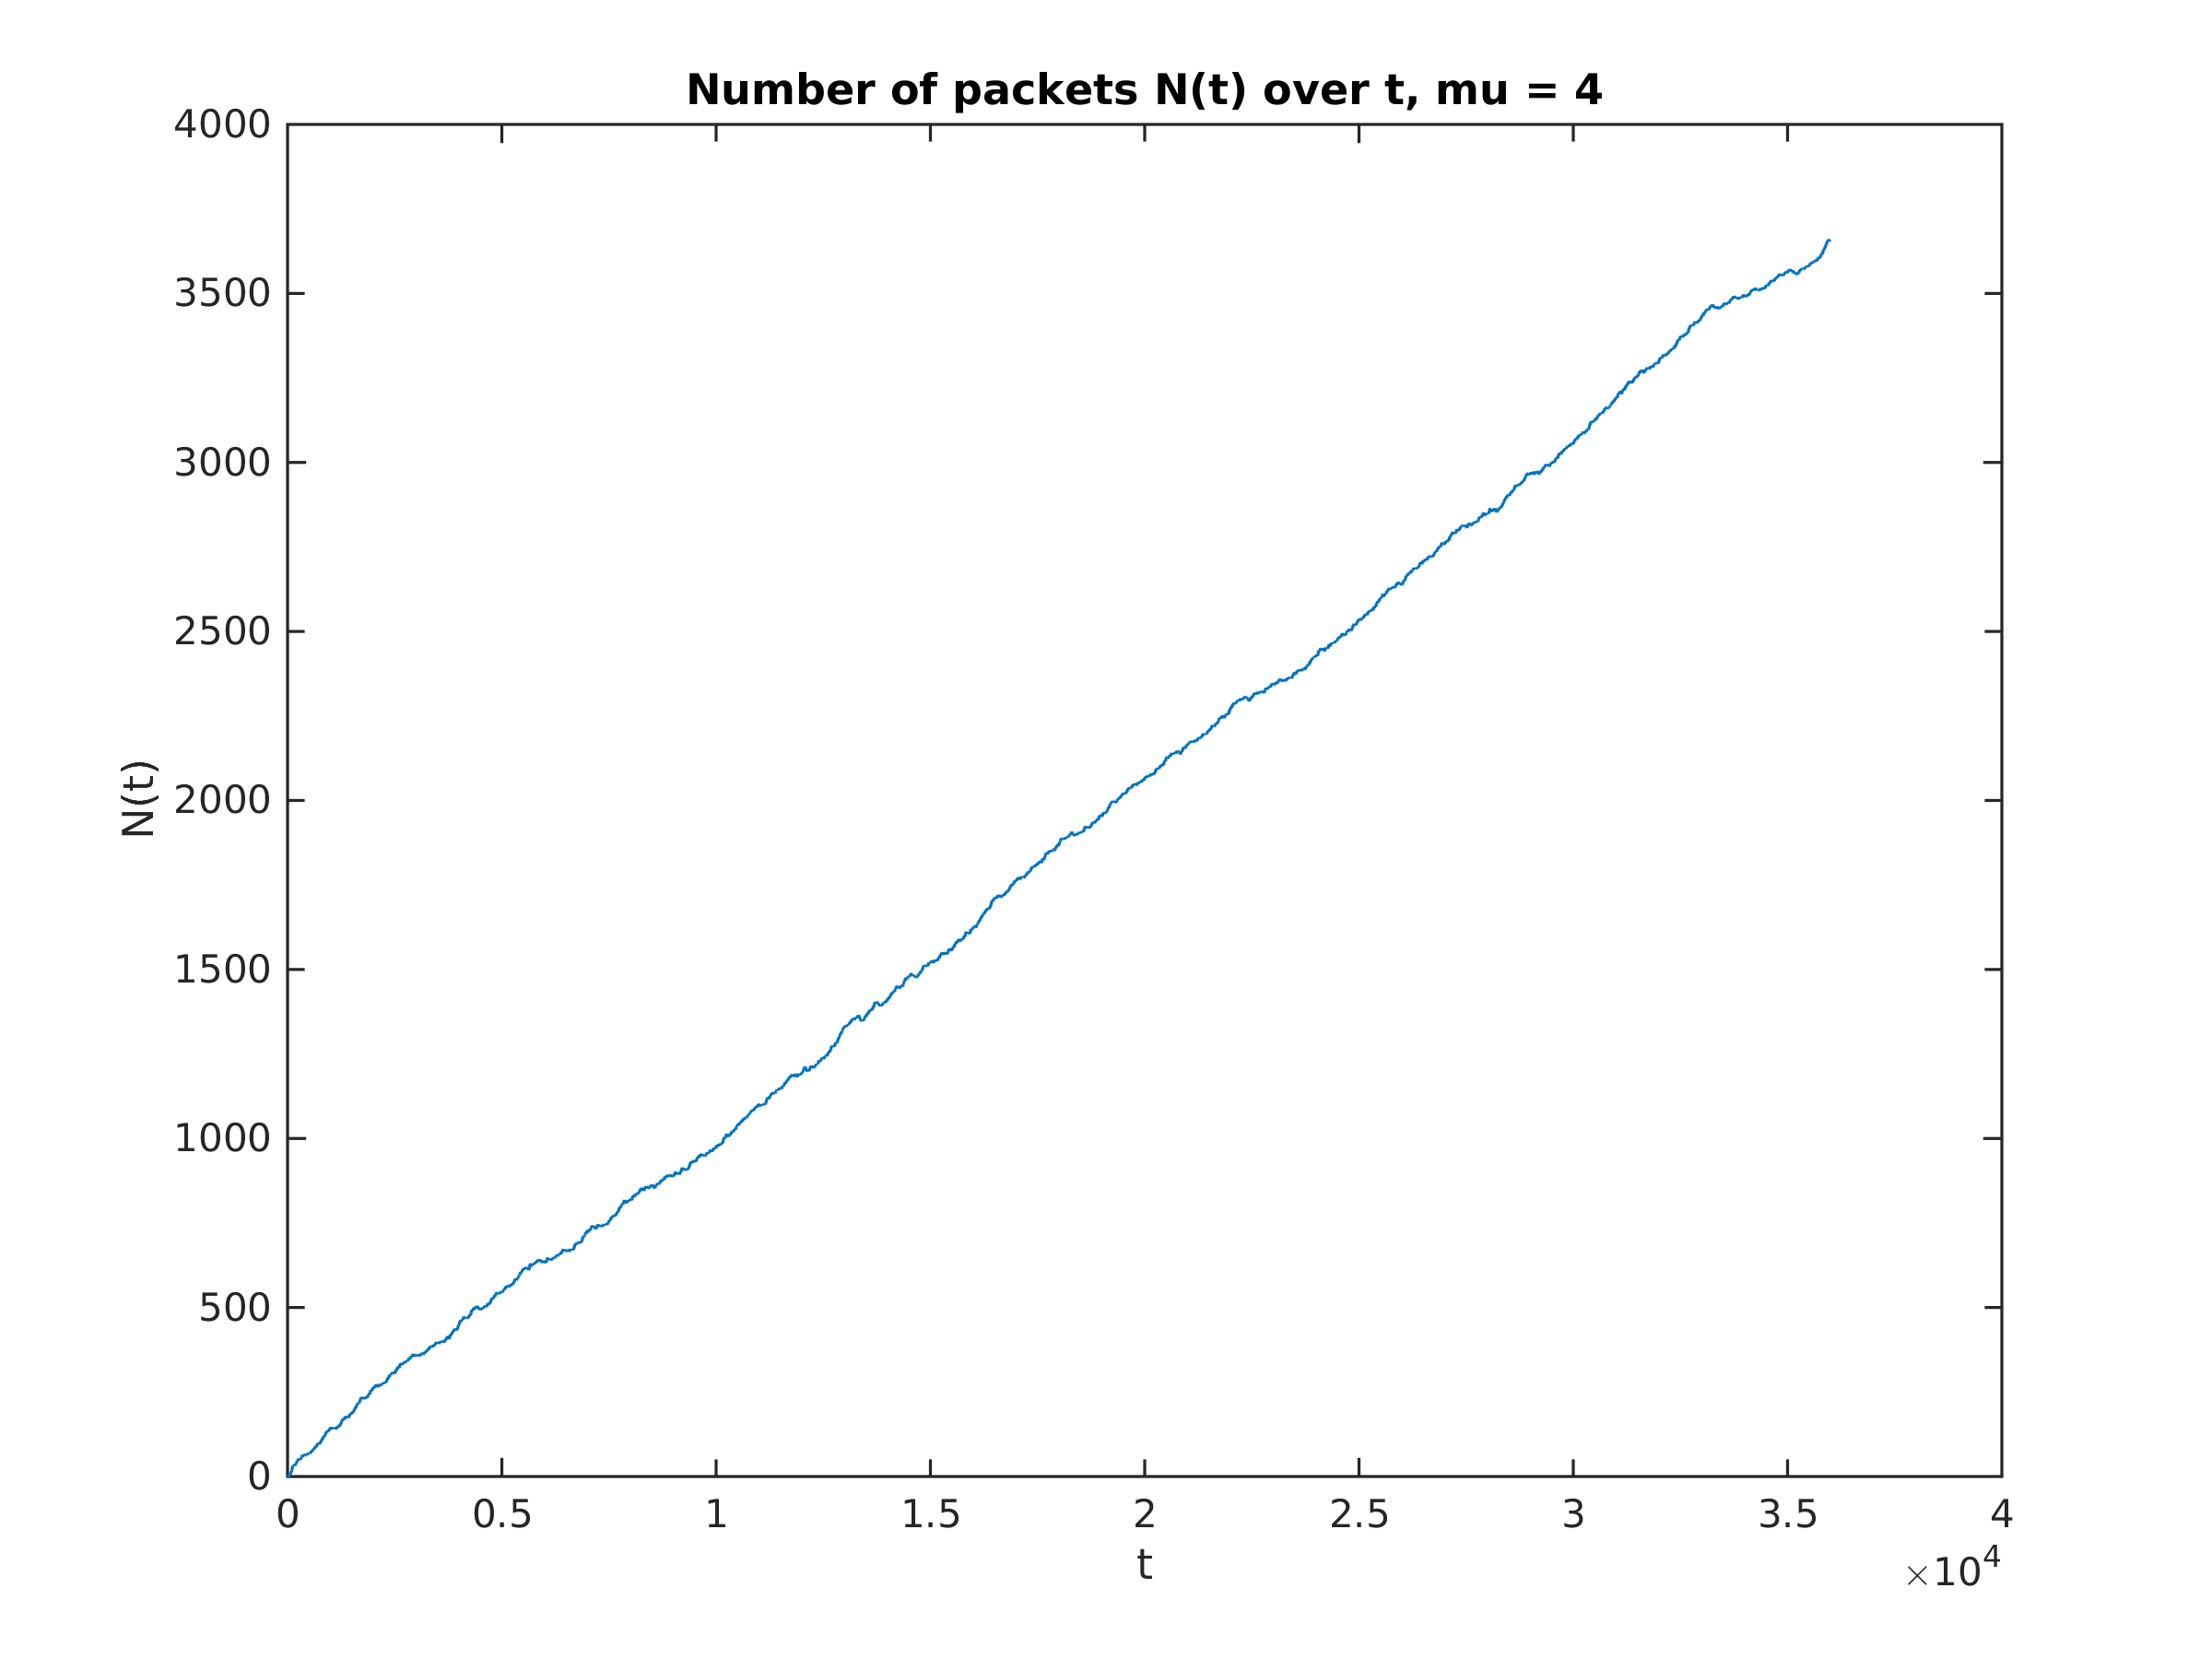
\includegraphics[width=1\linewidth]{hw3_3_nt_m4.png}
				\caption{$n(t)$ when $\mu = 4$.}
			\end{subfigure}
			\caption{$n(t)$ for $\mu = 10$ and $4$.}
		\end{figure}

		\vfill

		\begin{figure}[!hbt]
			\centering
			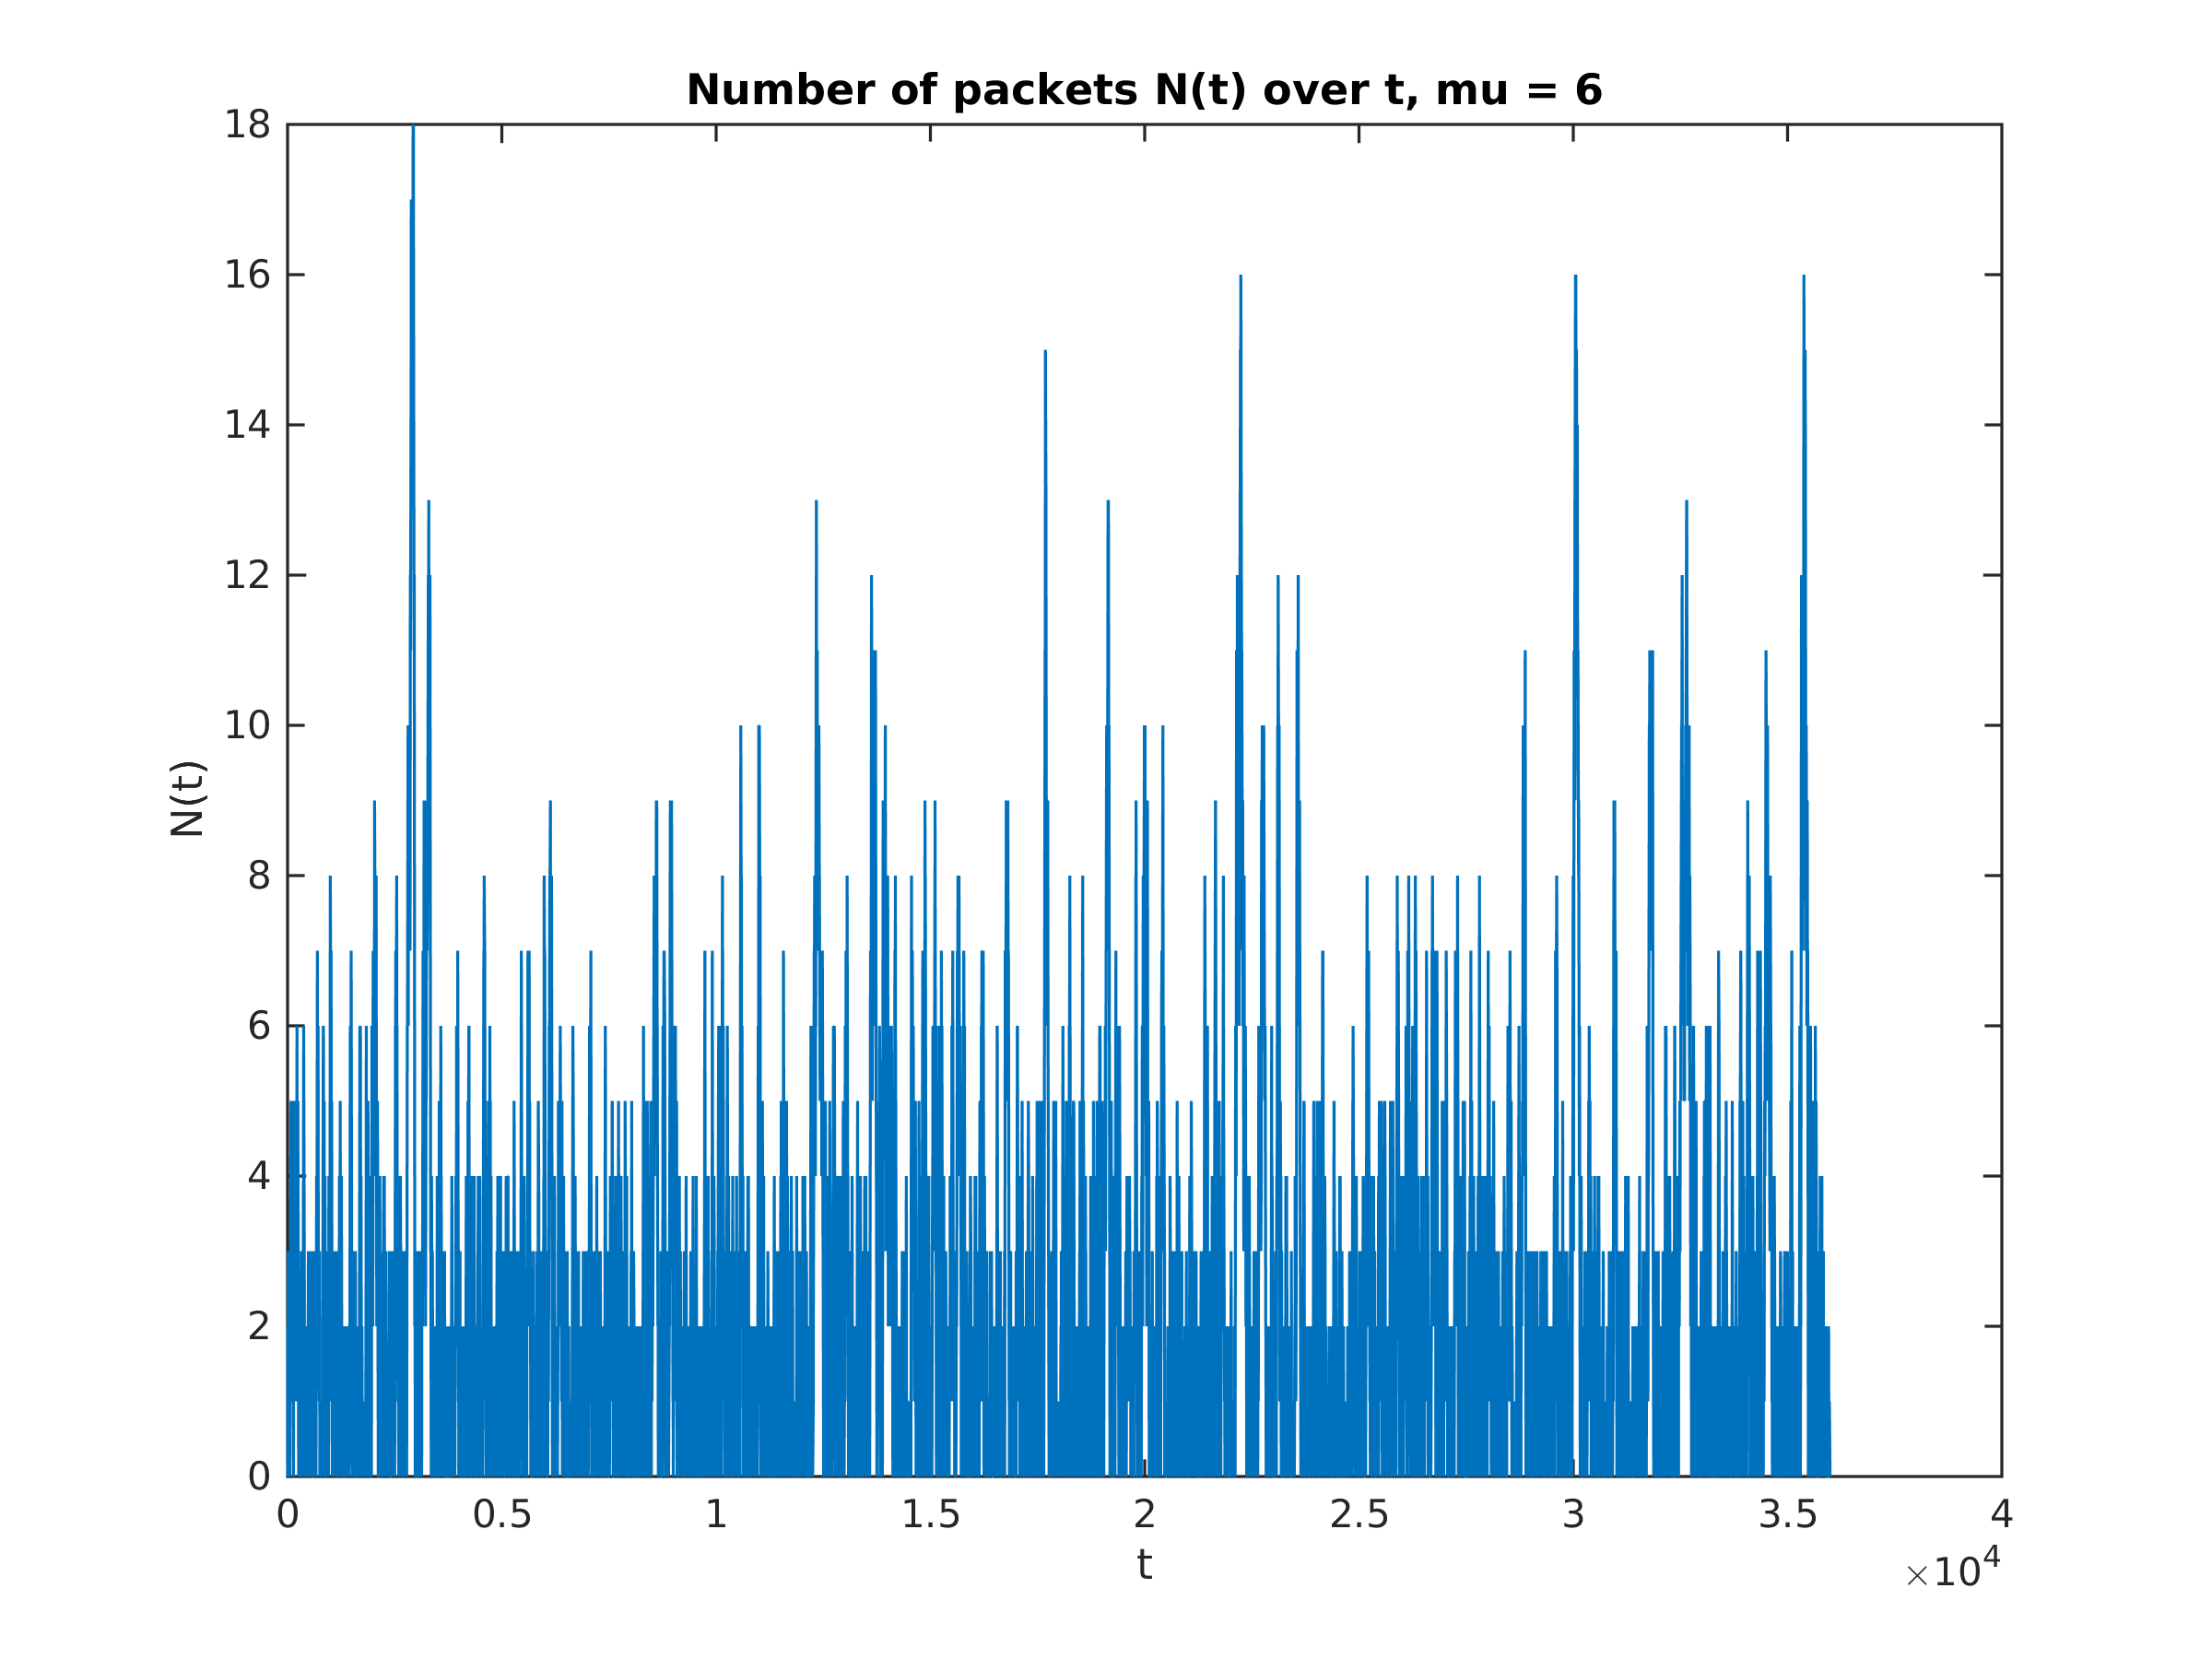
\includegraphics[width=0.5\linewidth]{hw3_3_nt_m6.png}
			\caption{$n(t)$ when $\mu = 6$.}
		\end{figure}
		\begin{figure}[!hbt]
			\centering
			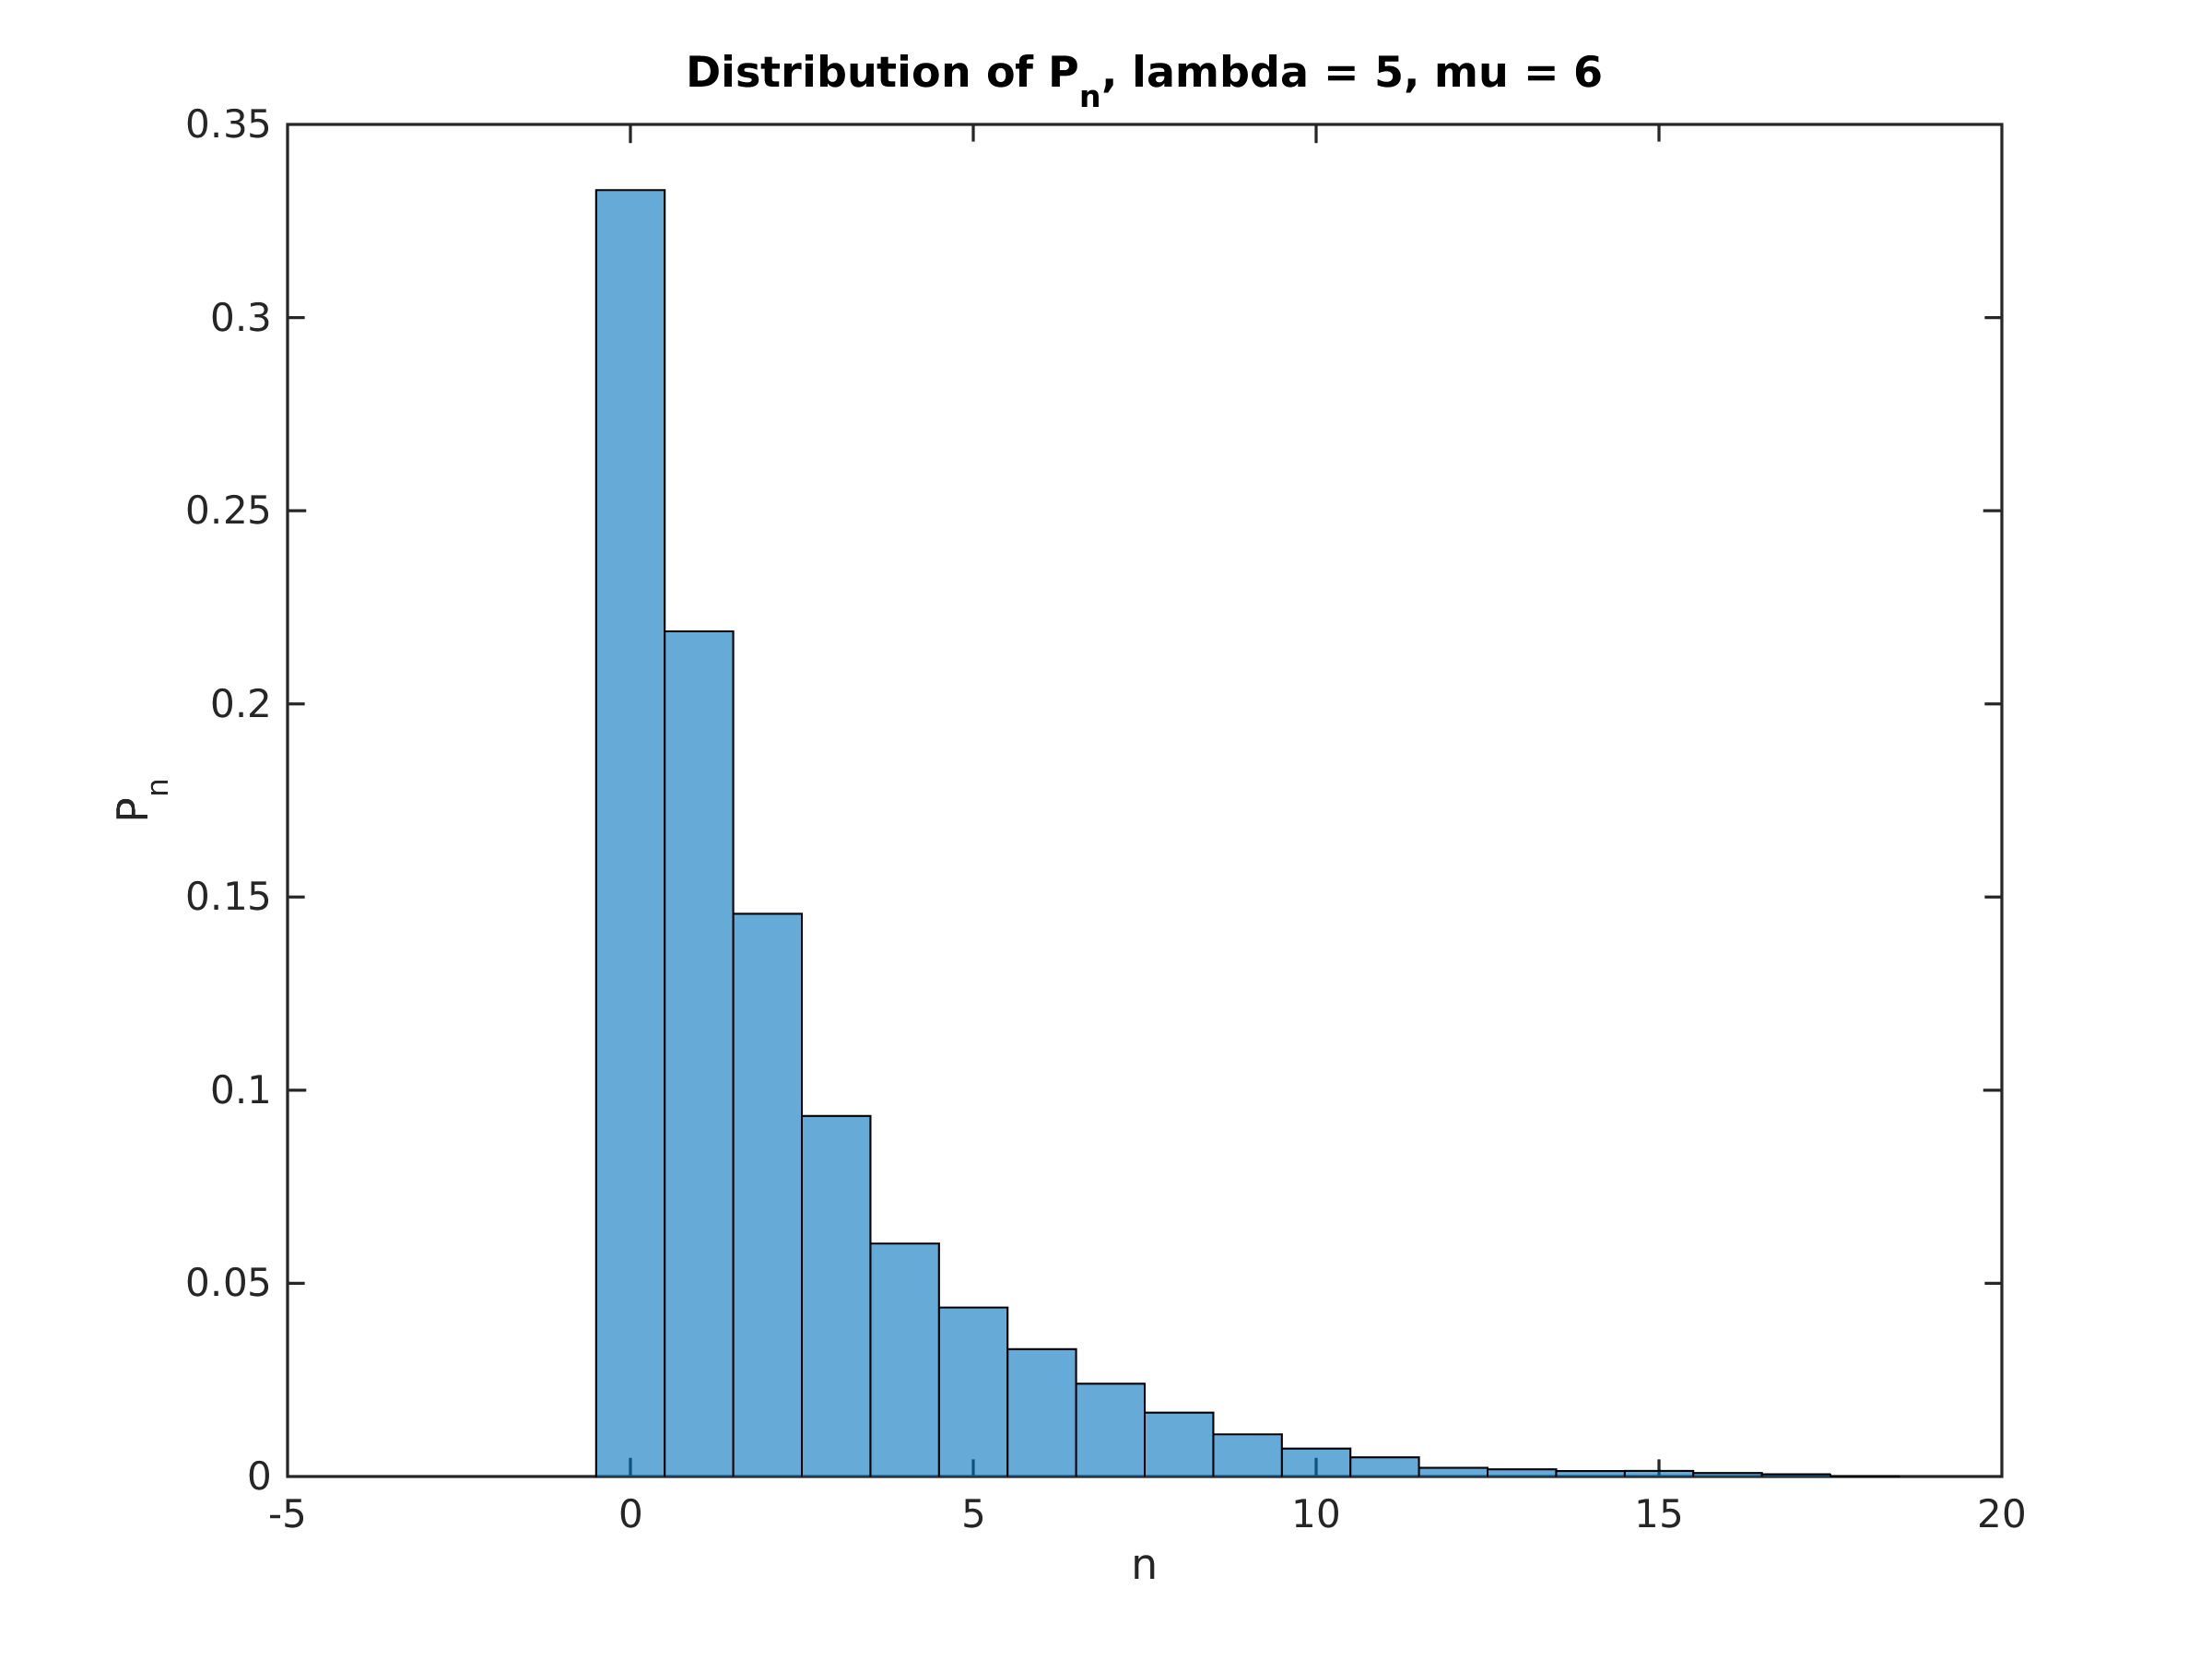
\includegraphics[width=0.5\linewidth]{hw3_3_pn_l5m6.png}
			\caption{Distribution of $P_n$ for all n.}
		\end{figure}


\end{document}
